\chapter{KWS and SV Models}
\label{cha:training}
\section{KWS Model}
\label{sec:kws deployment}
Keyword Spotting (KWS) is a model specialized in audio classification whose objective is to detect the presence of a spoken word or phrase according to an input sample, in this case the spectrogram extracted by MFE block. This transformation from raw data to spectrogram provides a time-frequency representation that emphasizes relevant acoustic features. A KWS model is trained to capture a predefined keyword by learn its spectral patterns across a range of samples, which must be differentiate and of a big size to ensure generalization across speakers and noise conditions.
In this thesis, the KWS model is destined for deployment on the Syntiant NDP101 hardware. Due to the hardware constraints and design recommendations given by Syntiant, a DNN architecture has to be employed with a maximum output of 64 classes. This network has 3 hidden fully connected layers and one output layer, used along with a softmax activation, mapping the feature vector into a probability distribution over defined class labels. The neural network structure strikes a balance between efficiency and classification accuracy, making it suited for real-time applications on embedded devices.
The focus in this work is on system verification, allowing to make a simple model consisting of one word, basically creating a binary output, that word or not. The chosen keyword for training is Sheila, chosen due to its availability within the Google Speech Commands dataset \cite{speechcommands}. This offers a substantial number of audio recordings designed for keyword classification research, including various samples from multiple speakers with varying environmental conditions.
The recordings in the dataset align with the Syntiant NDP101's input specifications, because they are sampled at 16kHz and have a one second duration per sample. In addition to the sheila’s samples, a good dataset should include a variety of background noise sounds, samples of words non present in the dataset and others similar phonetically, which may look similar for the neural network perspective. To give more samples as possible to the dataset, some audio clips were manually recorded or sourced from a dataset curated by Edge Impulse \cite{edgeimpulse_dataset_499022}, which is a platform specializing in machine learning for model developing and deploying on edge devices. It is important to note that in the dataset provided there are some Sheila samples, so to avoid any error in splitting is suggested a checking.
The final dataset used consists of 3403 sheila-words (almost 56m 43s of audio recoding). These samples were divided 80\% for training and 20\% for evaluation. This division ensures that meaningful representations are learnt while it is still providing independent data for validation.
To facilitate deployment on NDP101, the model is developed and trained using the Edge Impulse Studio\cite{edgeimpulse_kws_example}, which provides a good and intuitive pipeline for building and optimizing models tailored to the embedded hardwares. The processes done by this framework include automatic data preprocessing, training, fine-tuning, and a quantization model conversion to int4, which is compatible with the Syntiant device. This workflow reduces development time, ensuring at the same time that the resulting model fits in the memory.
During and after training, confusion matrices are generated for classification performance. These provide insights into which keywords were misclassified, highlighting potential areas of confusion and suggesting model refinement. They are useful in identifying failure cases, such as a confusion between similar-sounding words and to avoid this inconvenience, these words were already added to the dataset as other.
\begin{center}
  \begin{figure}[!h]
  \centering
  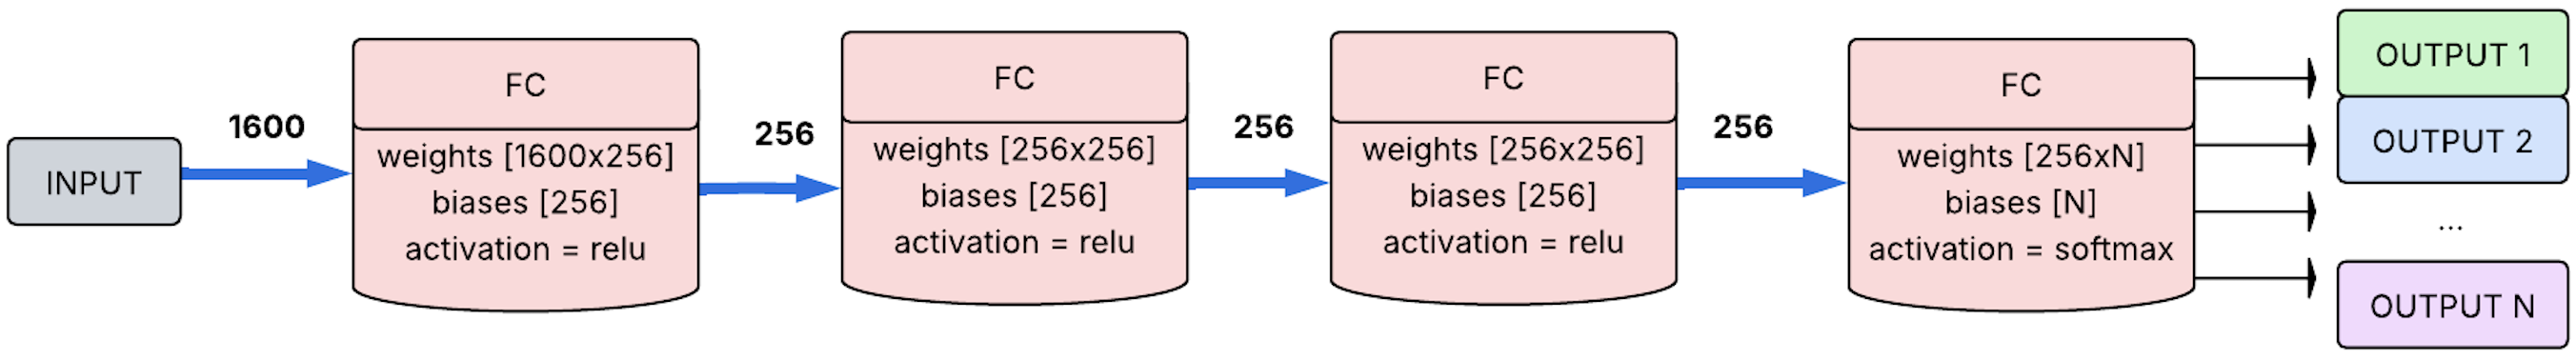
\includegraphics[width=1.0\textwidth]{images/3.01 KWS Model.png}
  \caption{Keyword Spotting Model}
\end{figure}
\end{center}
\section{SV Model}
\label{sec:sv introduction}
After creating the KWS model, the objective is creating a text-dependent Speaker Verification model, which requires only one train. This is known as ASV (Adaptive Speaker Verification), which relies on comparing the results of the model (d-vectors) with reference samples stored in system dataset, which have to be captured during inference phase. Speaker Verification is used in recognizing the identity of a user in a on-device learning context. To approach this way a large amount of data is required at first to train the model, performing a meticulous extraction of d-vectors to recognize patterns in user voice and possibly trying to minimize the required number of samples, maximizing the security recognition. A sample, because of text-depencendy, will correspond to a word said by one user and should compare only with its similar.\newline
The deployment of the model requires 3 caveats:\newline
1. Adapting directly on device, meaning that a new user should be able to enroll in SV application by providing samples of its voice in real time through the target device\newline
2. The algorithm has to operate in one-class manner and it should be able to learn to distinguish between the enrolled user and the others, only using the data from the dataset collected during inference\newline
3. To be fit in a TinyML device the considerations should be done in memory allocation depending on the device used, so the model should fit in Flash Memory\newline
To obtain the desired d-vector we should use a convolutional neural network, because we would like to reduce dimensionality, while obtaining significantly features. This is achieved with some expensive filters that while reducing width and heights, will generating new channels corresponding to a new feature extracted. This is a way to synthesize the input spectrogram (40 width x 40 height x 1 channel) to a lower dimension.\newline
A valid alternative, in theory, could be i-vectors. It is a feature that represents the characteristics of frame-level features distributive pattern. The extraction is a dimensionality reduction of GMM supervector, allowing an extraction per sentence, instead d-vector generates one-hot speaker label on the output and it is an averaged activation from the last hidden layer of CNN. The advantage of d-vector is that there is no assumption on feature's distribution, instead i-vector assumes as default a Gaussian distribution.
\subsection{D-Vector Extractor Creation}
\label{subsec:d-vector extractor creation}
The structure of the CNN follows the theoretical one introduced and as input is given the spectrogram given in output from MFE block (40x40x1) and as output the objective is a 256-size long array of relevant features (d-vector). However, it cannot be the model output, because at first the model should classify the data given in input, through a fully connected layer. As input dataset is used a huge one with many different speakers and each providing various samples, because they comes from audio book recording. From speakers classification is not required the text-dependent approach, so the speakers will say many different words, which helps in generate the required weights and biases for the convolution layers. The dataset used was from libreSpeech which has data collected per speaker and for the purpose was taken the one with 100 hours clean speech in English Language sampled with 16kHz, which is the same of Syntiant audio processing\cite{librispeech}, corresponding to ~6GB memory space to make the training successful in reasonable times.\newline
A first problem is that these samples are not already in 1 second, but variable, so they have been sampled and the parsed through the MFE Block previously introduced. The total spectrograms obtained were 136112 for a total number of classes of 94 and a total of ~38 hours of recording and a memory occupation of 871MB. To have a balanced dataset all classes had the number same samples 1448 as fact at first should have been 100, but they had too few samples. A convolution Neural should perform 3 actions during its creation in which the dataset should subdivide its samples:\newline\newline
1. Training - The spectrogram is threated as an image, this dataset is the base of the model and on these the weights are adjusted using backpropagation, like Adam optimizer, and using loss functions like cross-entropy, for classification, or MSE, for regression, to minimize the failure rate. It uses a learning rate, which is a hyperparameter, determining the step size at each iteration while moving forward with epochs. A epoch consists in a cycle of training input processing and an evaluation and can be arbitrary set according to the complexity of the network. In this case, it was set to 700.
2. Validation - This is used to see the result on data other than the ones in training set. It is used to adjust learning rate and batch size in case it starts overfitting or perform an early stopping if validation loss increases.\newline
3. Testing - It is a dataset to which are added background noise, varying microphone quality and other modifications to the original input. It is like a validation, but is to stress-out the system and seeing if it can still working with some fluctuations.\newline\newline
The distribution among these 3 sets is random inside a class, but each one will have an amount in each set. For precision, 70\% of samples will go in training (95278), 15\% in validation (20417) and 15\% in testing (20417). In training with CNN is suggested to avoid fluctuations a batch size and considering that the samples may not be complete words it performs an attenuate on those cases and the objective in having a good identification of the speaker. Knowing that a higher batch size will provide more accuracy, it was chosen 32 size, which should be stable with standard learning functions.\newline
The setup of the model, as summary, is an input shape of (32,40,40,1) [batch,width,height,channel] for 2977 inputs (95278/32) and output shape of 94 classes. The model creation required about 3 hours using a GPU. The proposed architecture is the following\cite{dvector_extractor_TinySV}:
\begin{center}
    \begin{figure}[!h]
        \centering
        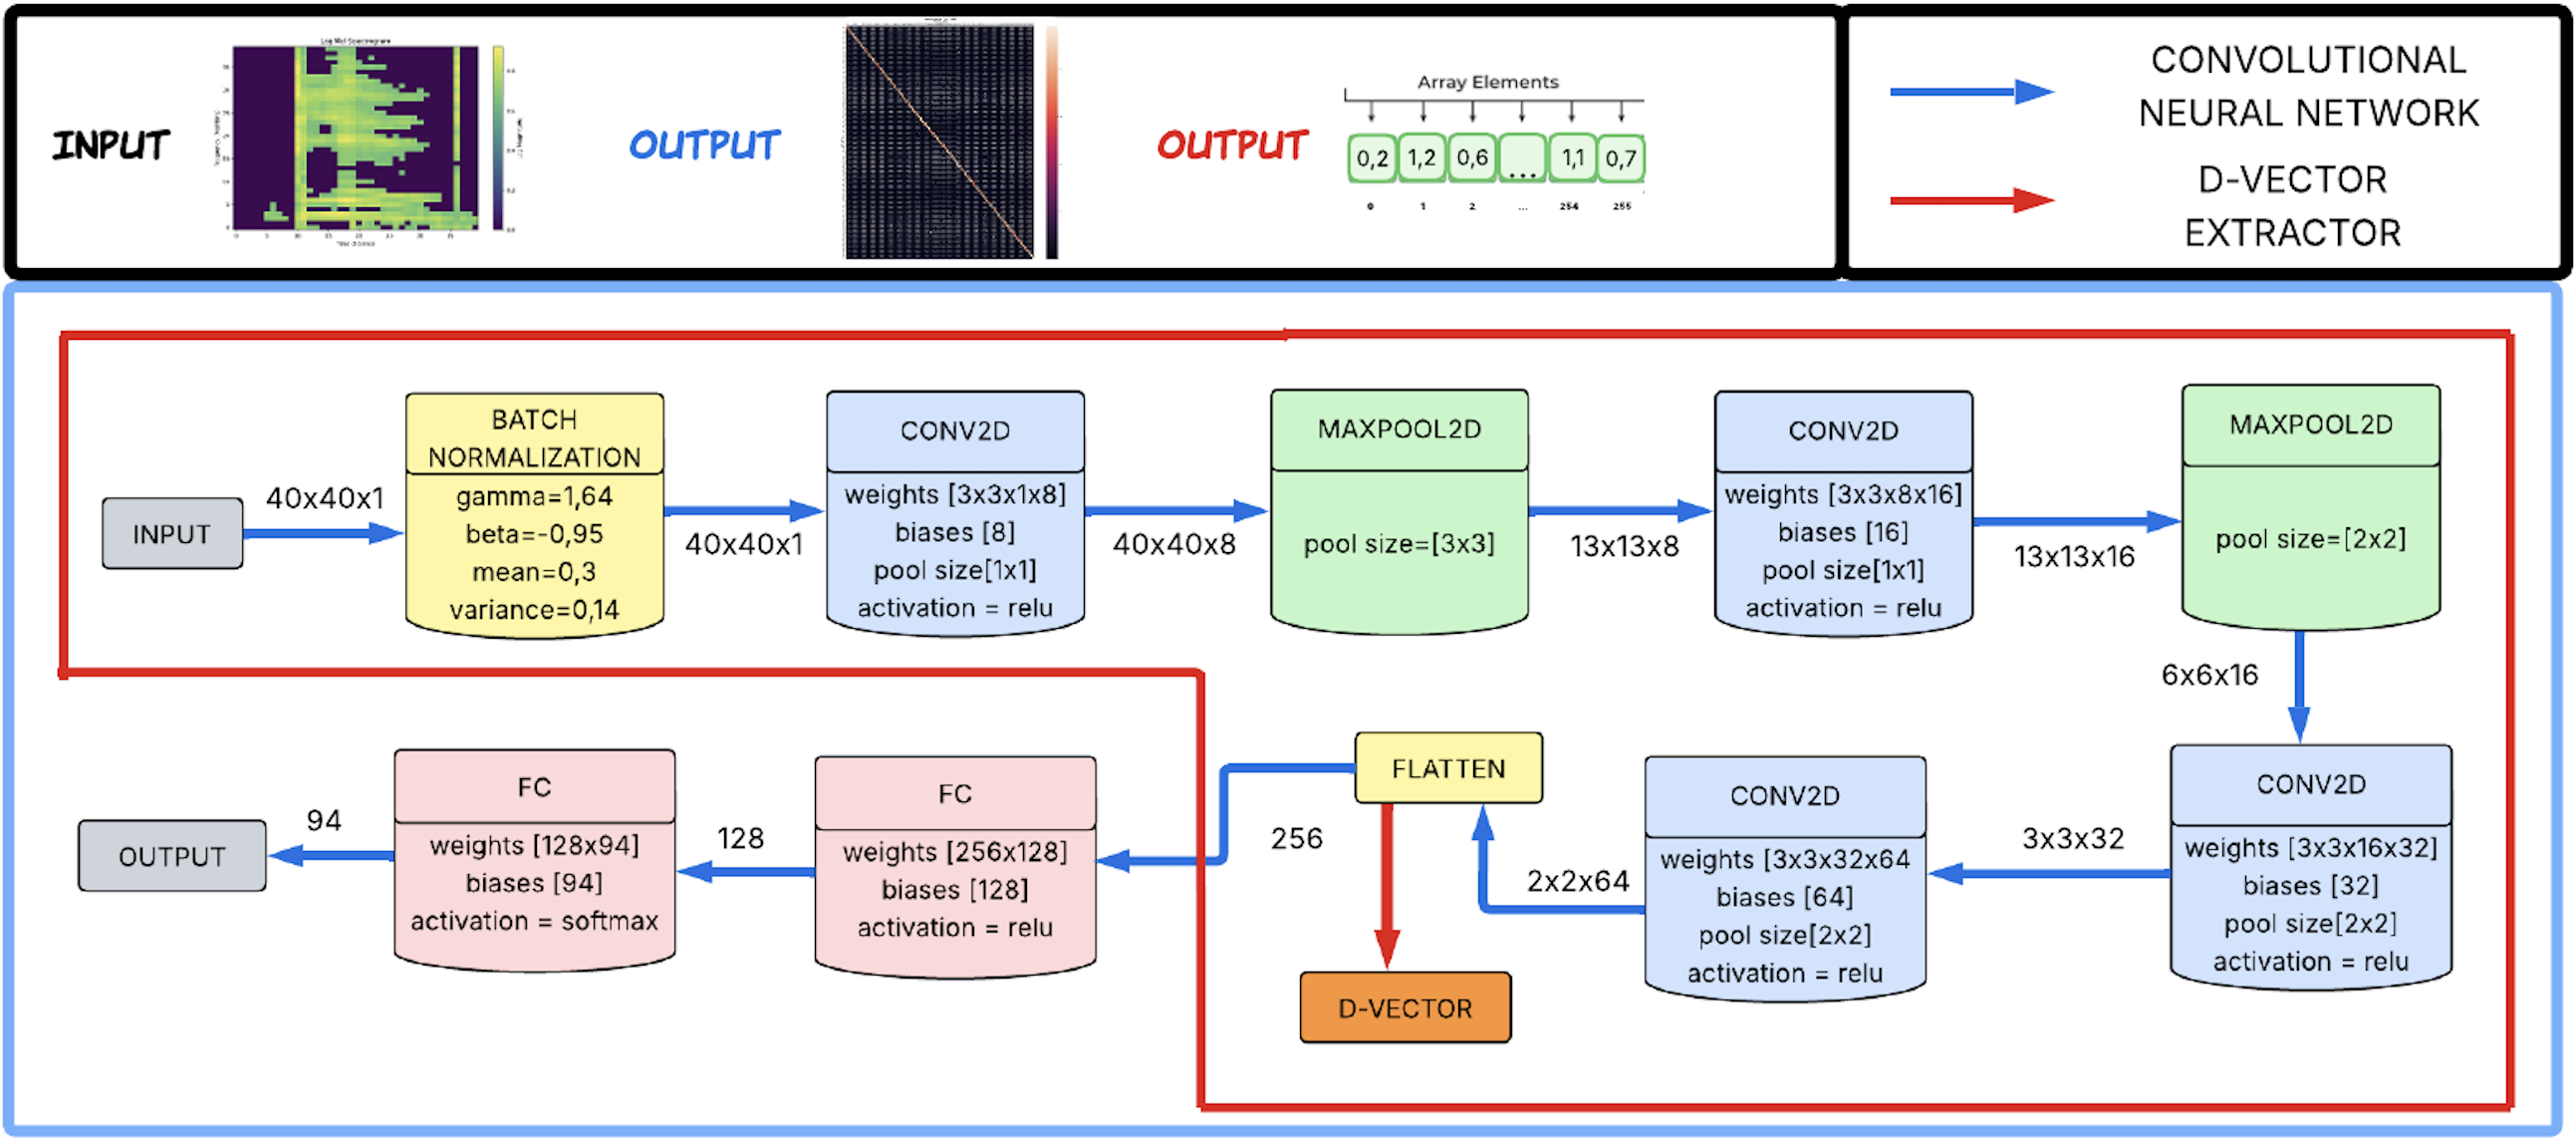
\includegraphics[width=1.0\textwidth]{images/3.02 D-vector Extractor.png}
        \caption{Speaker Verification Neural Network and D-vector Extractor}
    \end{figure}
\end{center}
After obtaining the CNN, we implemented the Fully Connected Layers to catalog and what is expected is even with 700 epochs and 32 batch, to have a good accuracy, but a bad loss, because we are trying to find patterns between very different samples. However, before the classification, so the Fully Connected layers, there is a generalized array of 256-size that represents the concept of d-vector, a general array that is a compression of the initial spectrogram and with max-pooling leverage relevant features, preserving all its consistency. Knowing this, we could truncate the DNN part of CNN and set the flatten section as the output and it is possible because the two logic are separated.\newline
The problem that will arise now is how can the accuracy be computed, because before it all depended on classification, but truncating that last part is required another method to capture that value and because this is an ASV model, it will not be trained again and if it was for a fixed user for a specific usage it would have been reasonable, but in this case it is not the solution. A notion that was introduced before consisted in cosine similarity. It takes two vectors and gives a percentage output on how much they are similar. The model that has just been created can provide a relevant reference of the audio sample given in input and if in a dataset a similar one is provided, even if the spectrogram are not identical with feature compression and filtering they will be very similar. There are some existing solutions on which the evaluation of the models was performed:\newline
1. Best-matching: During inference, the reference samples have to be recorded in real-time. It is recommended, because of this, to accept more than one sample and typically increasing the number of samples saved, more it is probable to find similar user samples. The best-matching technique saves per word said per user a number of vectors equal to the recommended size. It is important to notice that because the d-vector elements are floats, a single reference vector occupies 1KB.\newline
2. Mean Reference: Instead of saving all the reference samples, occupying N KB per user's word enrolled, to save space can be computed an average one. Theoretically, we would not have an optimal cosine similarity, however it is a good trade-off in space saving and considering the operation on a TinyML the minimizing of storage and memory allocation is important.\newline
In the case of Syntiant NDP101, because of the really low space is highly recommended to use mean reference technique to minimize power consumption.
\subsection{Knowledge Distillation Training}
If the solution may be deployable on some TinyML, it is not optimized and not compatible with Syntiant NDP101, because it can only support dense fully connected layer (DNN), but the d-vector extractor is a CNN\cite{distillation_from_cnn_to_dnn}\cite{knowledge_distillation}. Exists in machine learning a process called Knowledge Distillation. It adapts two different models with even different architecture, but with equal input and output data. To perform this, there should be a teacher and a student model. The teacher is CNN and is taken and the student is DNN that tries to replicate the results of the teacher at feeding of input data. The orientation of the student will be the loss discrepancy being 1-cosine similarity. To evaluate the model can be used both cosine similarity, but Mean Square Error is a solution, too. The advantages of this kind of approach is not only for deployment on NDP101, but dense layers have an easier computation than convolutional layers, which require more power consumption. As a consequence, the model would be faster. However, it should require more parameters to obtain similar results, because 3 hidden layers structure remains fix. In definitive, the model would be less precise and occupy more memory, but will be more faster and deployable on NDP101.
\begin{center}
\begin{figure}[!h]
        \centering
        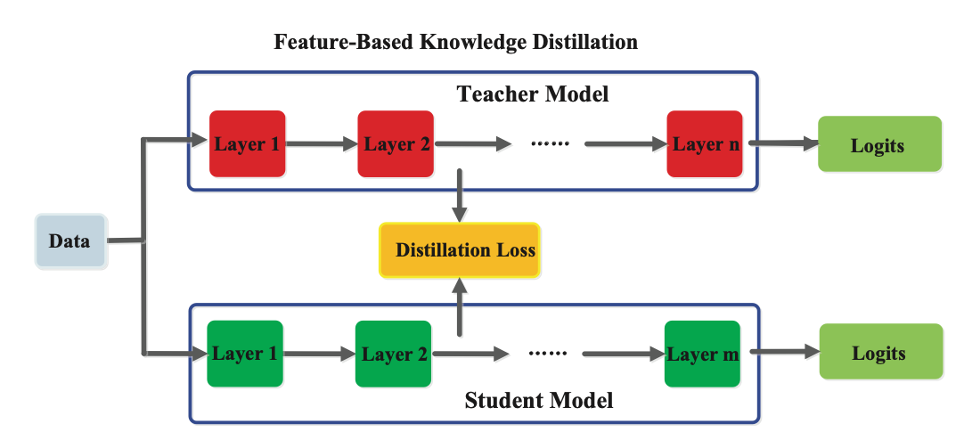
\includegraphics[width=1.0\textwidth]{images/3.03 Distillation Technique.png}
        \caption{Distillation Model from CNN to DNN}
    \end{figure}
\end{center}
The number of neurons per layers have to be chosen by the user, but there are some caveats to consider:\newline
• Syntiant NDP101 supports at most 589.000 parameters, so the neuron choice must be taken in account\newline
• Downscaling and then upscaling between two layers is not recommended and there should be a reduction in results performances\newline
• The neurons typically are multiples of 2 to optimize space, in case that would be too inefficient is recommended to take at least multiples of 2's multiples.\newline
\subsection{Quantization of SV Model}
\label{sec:quantization}
\begin{wrapfigure}{r}{0.35\textwidth}
  \begin{center}
    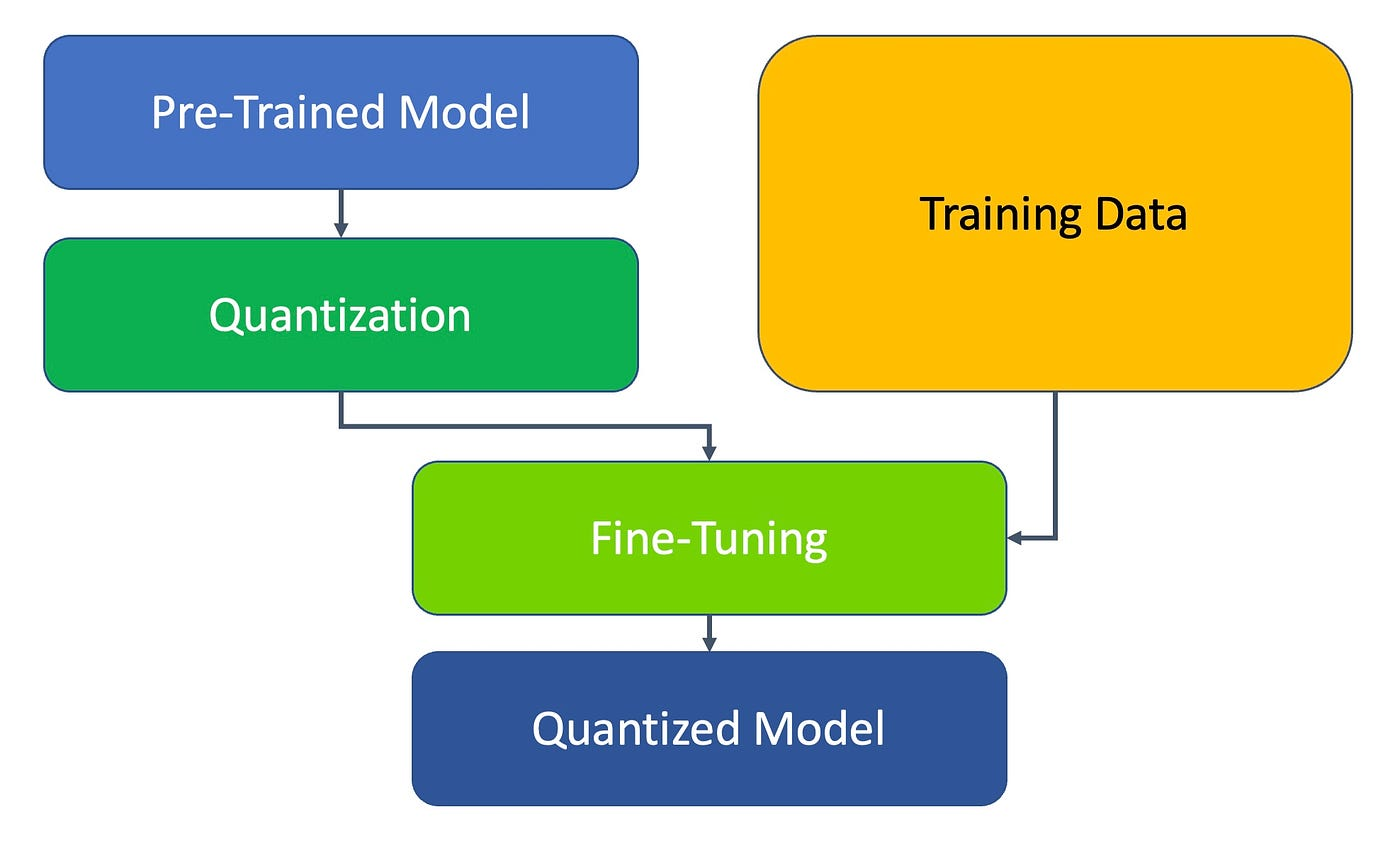
\includegraphics[width=0.35\textwidth]{images/3.04 Quantization Flow.jpg}
  \end{center}
  \caption{Quantization with Tensorflow}
\end{wrapfigure}
Unfortunately, the problems do not end here. Syntiant NDP101 not only has a DNN, but requires a parameters' quantization, too. The weights should be stored in 4-bit\cite{description_ndp101} integers, meanwhile biases in 32-bit integers. Performing a quantization is the most straightforward way and in case of transposing it to int-8 it is immediate, thanks to support provided by Edge Impulse with Post-Quantization-Training (PQT)\cite{pqt_tensorflow}, which is the case considering that the distilled model is trained. However, the int-4 quantization is not optimized and as of now consists in a fake int-4 quantization, like storing in int-8 bits allocation int-4.\cite{wu2023understandingint4quantizationtransformer} But, can be seeing that PQT int4 weights has really poor performances. Instead, and performing a Quantization-Aware-Training (QAT)\cite{qat_tensorflow} as of now can achieve decent results, always using fake-quantization. The problem is that it's unknown how the Syntiant binary is built and composed, so even with a good packing-unpacking technique, it could be difficult to obtain something from the model. Syntiant NDP101 provides a tool with the SDK to convert a model into binary Syntiant compatible, but it is under NDA. A solution could be using using Edge Impulse Framework, but it supports only classification and regressions models as of know and it is not what the d-vector extractor is performing.\newline
However, in theory, to successfully quantize the model it has to be performed a brute force quantization and then a fine-tuning to adjust values passing database data. An advantage of this, is the size of the model, not only the weights are adjusted, but the intermediate input and output layers, too, leading in having an output no longer of 1KB, but of 256 bytes. It will save even more space in memory, however to be sure to convert the input spectrogram in int, the model can be fake-quantize to leave the input and the output as floats adding a quantize and dequantize layer, the ones inside will be int8 and then remove manually from dequantize layer. This will allow to maintain the float spectrogram logic, but at the same time allowing inference on Syntiant, if the conversion tool was available and saving memory because of the reduction of 75\% per sample.
\begin{center}
\begin{figure}[!h]
        \centering
        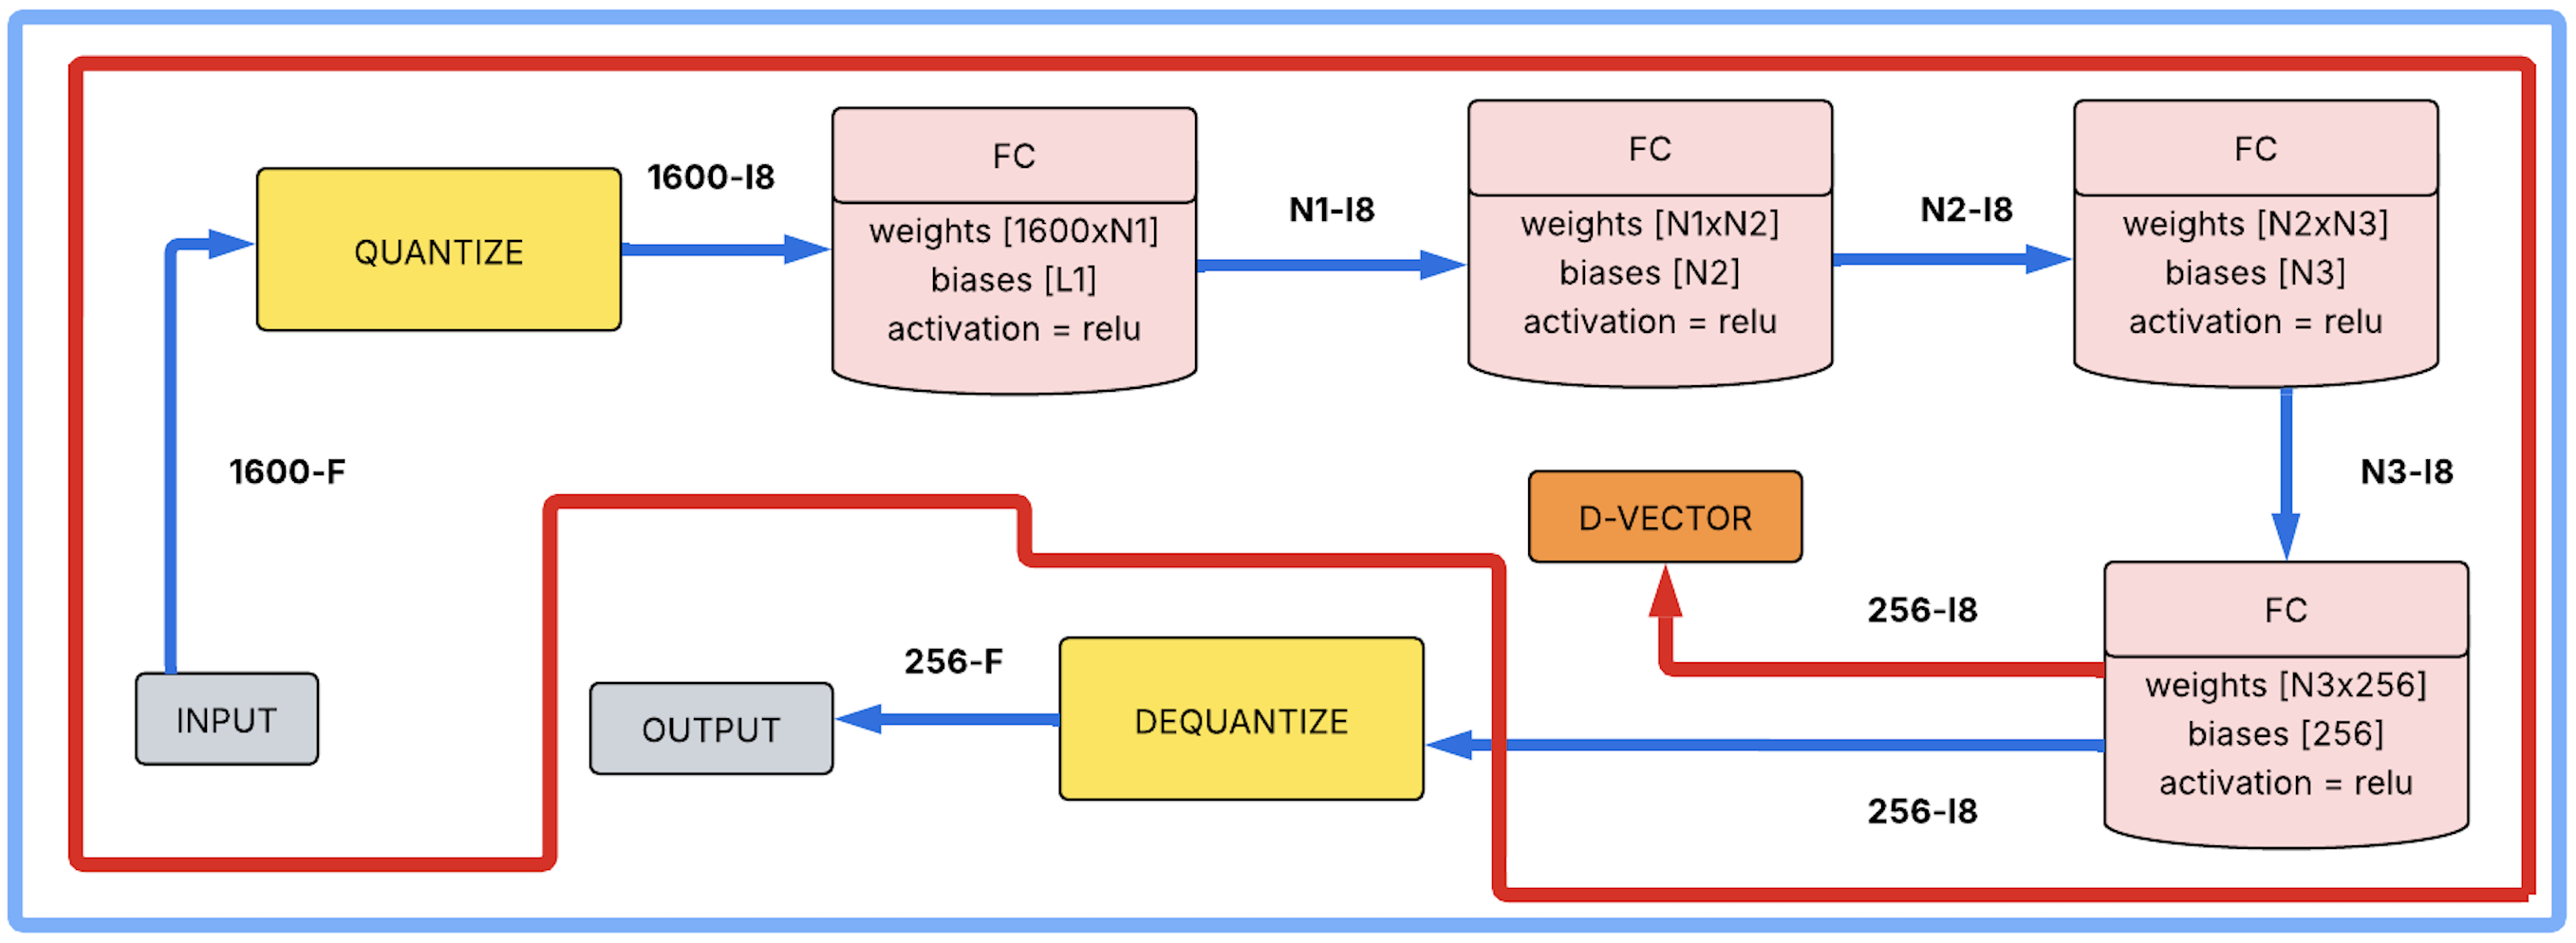
\includegraphics[width=1.0\textwidth]{images/3.05 Quantized Model Int8.png}
        \caption{Quantized Model Int8}
    \end{figure}
\end{center}
\newpage